\section{Method}\label{sec:method}

In \method, the model learns from the execution of its own sampled queries
on the client databases. In each preference round, a client samples SQL
queries from the current global model, executes them on its databases,
labels them by comparison with the execution result of the gold SQL query
and trains on pairs of a correct and an incorrect sample of the same
question.

\subsection{Problem Formulation}\label{sec:formulation}

We consider $K$ clients. Client $k$ holds a training set $\mathcal{D}_k$
of $n_k$ elements $(q, d, y^\star)$, each consisting of a question $q$, the
database $d$ on which it is posed and its gold SQL query $y^\star$. None
of them leaves the client. The clients jointly train one model: the
pretrained model is frozen, and a LoRA adapter $\theta$~\cite{hu2022lora}
is the only set of parameters that is trained, communicated and
aggregated. We write $\pi_\theta$ for the model with adapter $\theta$. The
prompt $x$ contains $q$ and the schema of $d$ as \texttt{CREATE TABLE}
statements. On Spider each statement is followed by up to three rows of
its table, and on BIRD the prompt adds the external knowledge that the
benchmark attaches to the question (Fig.~\ref{fig:prompt},
Appendix~\ref{app:prompt}). The same prompt serves training, sampling and
evaluation. Training runs for $T$ rounds, all $K$ clients participating
in each. In round $t$, the server sends the global adapter
$\theta^{t-1}$, client $k$ obtains $\theta_k^{t}$ by local training from
$\theta^{t-1}$ with a newly initialized optimizer, and the server
aggregates the client adapters into $\theta^{t}$.

FedAvg SFT~\cite{mcmahan2017fedavg,ye2024openfedllm} trains the adapter
on the gold SQL queries. Client $k$ minimizes the token-averaged NLL of
the gold SQL query,
\begin{equation}
  \mathcal{L}_k^{\mathrm{SFT}}(\theta) = \frac{1}{n_k}
    \sum_{(q, d, y^\star) \in \mathcal{D}_k}
    -\frac{1}{\lvert y^\star \rvert} \log \pi_\theta(y^\star \mid x),
  \label{eq:sft}
\end{equation}
and uploads $\theta_k^{t}$ together with $n_k$. The server averages the
adapters with weights proportional to the numbers of questions:
\begin{equation}
  \theta^{t} = \sum_{k=1}^{K} w_k \, \theta_k^{t},
  \qquad
  w_k = \frac{n_k}{\sum_{j=1}^{K} n_j}.
  \label{eq:aggregation}
\end{equation}
In Eq.~\eqref{eq:sft}, the gold SQL query is the only target and the
database enters only as text of the prompt. During local
training the model generates no query, so no loss term is computed on a
query of its own. Neither the gold SQL query nor a query of the model is
executed, no execution result enters the loss, and nothing identifies
which of the model's queries are incorrect.

\subsection{Execution-Derived Supervision}\label{sec:supervision}

A SQL query is verifiable by execution. Let $\mathrm{exec}(y, d)$ denote
the execution result of a query $y$ on the database $d$. For an element
$(q, d, y^\star)$, a query $y$ that the model generates for $q$ can be
labeled correct or incorrect by comparing $\mathrm{exec}(y, d)$ with
$\mathrm{exec}(y^\star, d)$. Execution thus turns the single gold SQL
query of a question into many labeled queries of the model's own,
incorrect ones among them. We refer to the training signal that these
labels provide as execution-derived supervision. It requires both $d$
and $y^\star$ and can therefore be computed only at the client.

On BIRD, this signal is available for most training questions. In the
BIRD setup of Section~\ref{sec:fed-setups}, \setting{pref.samples}
samples per question from the global model after
\setting{rounds.warmup} rounds of FedAvg SFT (Section~\ref{sec:labeling})
include both a correct and an incorrect sample for
\fact{cost.bird.pref1.paired_pct}\% of all
\fact{cost.bird.pref1.questions} training questions of the clients.

\subsection{Framework Overview}\label{sec:overview}

\begin{figure}[!t]
\centering
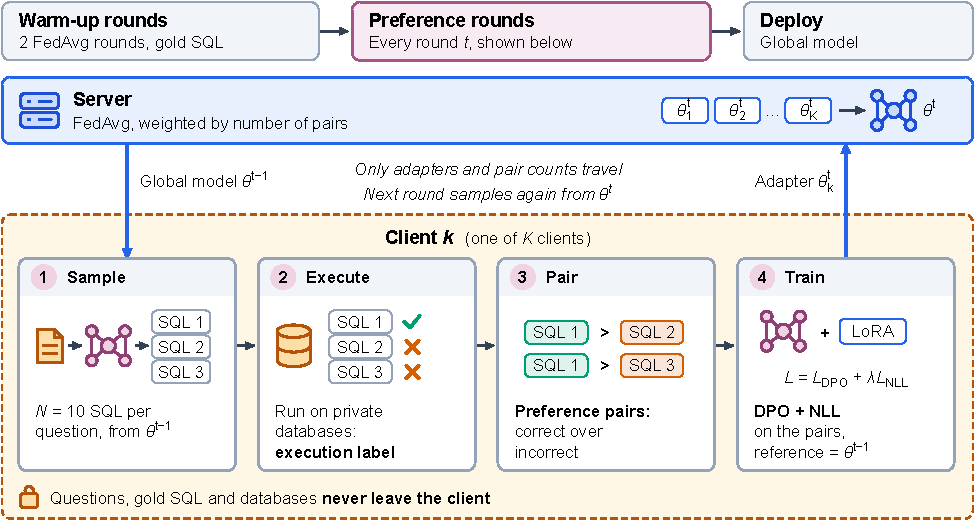
\includegraphics{figures/fig_method_overview.pdf}
\caption{Overview of \method. On the arrows, ``Global model
$\theta^{t-1}$'' denotes the global adapter, and ``count'' is $n_k$ in a
warm-up round and $\lvert\mathcal{P}_k^{t}\rvert$ in a preference round.
In step~1 and step~4, $\theta^{t-1}$ stands for the model
$\pi_{\theta^{t-1}}$, which is $\pi_{\mathrm{ref}}$ in
Eq.~\eqref{eq:logratio}. Step~1 shows the default setting
$N = {}$\setting{pref.samples}. In step~4, $L_{\mathrm{DPO}}$ and
$L_{\mathrm{NLL}}$ are the preference term and the NLL term of
Eq.~\eqref{eq:loss}.}
\label{fig:overview}
\end{figure}

We propose \method, a federated learning framework for Text-to-SQL that
trains on execution-derived supervision. It consists of four components
and an aggregation rule, organized into two kinds of round
(Fig.~\ref{fig:overview}, Algorithm~\ref{alg:method}) that differ in the
role of the gold SQL query. In the warm-up rounds $1, \dots, T_w$ it is
the training target, whereas in the preference rounds
$T_w + 1, \dots, T$ it is executed to produce the execution labels and
is not a training target. Every round ends with federated averaging of
the adapters. Supervised warm-up (Section~\ref{sec:warmup}) consists of
the warm-up rounds, which are rounds of FedAvg SFT. The other three
components make up a preference round: client-side execution labeling
(Section~\ref{sec:labeling}) samples $N$ queries per question from the
current global model and labels them by execution, on-policy pair
construction (Section~\ref{sec:pairs}) forms $M$ preference pairs per
question from these samples, and the preference objective
(Section~\ref{sec:objective}) trains the adapter on the pairs, with the
current global model as reference model. By default,
$T = {}$\setting{rounds.total}, $T_w = {}$\setting{rounds.warmup},
$N = {}$\setting{pref.samples} and $M = {}$\setting{pref.pairs}, with
\setting{sft.epochs} local epoch per warm-up round and
\setting{pref.epochs} per preference round. Table~\ref{tab:settings} in
Appendix~\ref{app:settings} lists the remaining settings, and
Section~\ref{sec:main} reports the resulting gain over FedAvg SFT
(Table~\ref{tab:main}).

\begin{algorithm}[t]
\caption{\method}\label{alg:method}
\begin{algorithmic}[1]
\Require training sets $\{\mathcal{D}_k\}_{k=1}^{K}$, pretrained model,
  $T$, $T_w$, $N$, $M$, $\beta$, $\lambda$
\Ensure global adapter $\theta^{T}$
\State initialize the adapter $\theta^{0}$
\For{$t = 1, \dots, T$}
  \State the server sends $\theta^{t-1}$ to all $K$ clients
  \ForAll{clients $k = 1, \dots, K$ in parallel}
    \If{$t \le T_w$} \Comment{warm-up round}
      \State $\theta_k^{t} \gets$ local training from $\theta^{t-1}$ on
        $\mathcal{D}_k$ with the loss of Eq.~\eqref{eq:sft}
      \State upload $\theta_k^{t}$ and $n_k$
    \Else \Comment{preference round}
      \State sample $N$ queries from $\pi_{\theta^{t-1}}(\cdot \mid x)$
        for each $(q, d, y^\star) \in \mathcal{D}_k$
      \State label the samples by comparing $\mathrm{exec}(y, d)$
        with $\mathrm{exec}(y^\star, d)$
        (Section~\ref{sec:labeling})
      \State $\mathcal{P}_k^{t} \gets$ $M$ pairs $(y^{+}, y^{-})$ for
        each question that yields pairs (Section~\ref{sec:pairs})
      \If{$\mathcal{P}_k^{t} \neq \emptyset$}
        \Comment{otherwise no update, $w_k = 0$}
        \State $\theta_k^{t} \gets$ local training from $\theta^{t-1}$
          on $\mathcal{P}_k^{t}$ with the loss of Eq.~\eqref{eq:loss},
          $\pi_{\mathrm{ref}} = \pi_{\theta^{t-1}}$
        \State upload $\theta_k^{t}$ and $\lvert\mathcal{P}_k^{t}\rvert$
      \EndIf
    \EndIf
  \EndFor
  \State $\theta^{t} \gets \sum_{k=1}^{K} w_k \, \theta_k^{t}$, with
    $w_k \propto n_k$ if $t \le T_w$ and
    $w_k \propto \lvert\mathcal{P}_k^{t}\rvert$ otherwise
\EndFor
\State \Return $\theta^{T}$
\end{algorithmic}
\end{algorithm}

\subsection{Supervised Warm-Up}\label{sec:warmup}

A preference pair needs a correct sample, and a question whose labeled
samples are all incorrect yields none. Measured as in
Section~\ref{sec:supervision}, this is the case for
\fact{warmup.bird.k0.no_correct} of the
\fact{cost.bird.pref1.questions} BIRD training questions under the
pretrained model. We reduce their number by supervised warm-up: in each
of the first $T_w$ rounds, client $k$ minimizes Eq.~\eqref{eq:sft} over
$\mathcal{D}_k$ and the server aggregates by
Eq.~\eqref{eq:aggregation}, as in FedAvg SFT. After
\setting{rounds.warmup} warm-up rounds, the labeled samples are all
incorrect for \fact{warmup.bird.k2.no_correct} questions. Neither count
includes the questions whose gold SQL query fails to execute or exceeds
the time limit, as their samples receive no label
(Section~\ref{sec:labeling}).

Warm-up is a setting of the framework, not a precondition of the
preference rounds. The adapter $\theta^{0}$
has the standard LoRA initialization, under which $\pi_{\theta^{0}}$ is
the pretrained model. With $T_w = 0$, the first round of
Algorithm~\ref{alg:method} therefore samples from the pretrained model,
which already yields preference pairs, and uses it as reference model.
Section~\ref{sec:ablation} examines the effect of $T_w$ on accuracy.

\subsection{Client-Side Execution Labeling}\label{sec:labeling}

In preference round $t$, client $k$ samples $N$ queries for each element
of $\mathcal{D}_k$ from $\pi_{\theta^{t-1}}(\cdot \mid x)$ at
temperature \setting{pref.t}, without nucleus or top-$k$ truncation and
with at most \setting{pref.tokens} new tokens per sample. It executes
each sample $y$ and, once per question, the gold SQL query $y^\star$ on
$d$, under the time limit of the benchmark's evaluation
(Section~\ref{sec:setup}). The execution label of $y$ is correct if
$\mathrm{exec}(y, d) = \mathrm{exec}(y^\star, d)$ under the comparison of
the evaluation metric, and incorrect otherwise. A sample that fails to
execute, reaches the time limit while it runs or contains no query is
therefore incorrect.

A sample has no label when its result is never compared with the gold
result. This is the case when the sample is cut at the token limit and
not executed, when the time limit is reached after
the sample has completed but before the comparison
(Section~\ref{sec:setup}), and when the gold SQL query fails to execute
or exceeds the time limit, which leaves the whole question without
labels.

\subsection{On-Policy Preference Pair Construction}\label{sec:pairs}

We construct the preference pairs $\mathcal{P}_k^{t}$ of client $k$ anew
in every preference round $t$, from that round's labeled samples.
FedDPO~\cite{ye2024openfedllm} instead trains each client on a fixed
preference dataset whose responses are not outputs of the model under
training. A question yields
pairs when it has at least one correct and one incorrect sample and some
table of its database contains a row. On a database without rows,
queries of different meaning return the same result, and a sample that
executes can match the gold result whether or not it is correct. We
exclude the questions on such a database, although their samples are
labeled (Section~\ref{sec:fed-setups}).

For each question that yields pairs, we draw $M$ samples uniformly from
its correct samples and, independently, $M$ from its incorrect samples.
Each draw is without replacement when the question has at least $M$
samples of that label and with replacement otherwise, and identical
queries among the samples are not merged. Pairing the two draws in order
gives $M$ pairs $(y^{+}, y^{-})$ per question, so that
$\lvert\mathcal{P}_k^{t}\rvert$ is $M$ times the number of questions of
client $k$ that yield pairs. We draw a fixed number of pairs per
question, rather than all combinations of its correct and incorrect
samples, so that every question that yields pairs carries the same
weight in the local objective. One local epoch runs over $M$ pairs of
each such question, and $M$ thereby sets the length of local training
per question.

With pairs constructed in every round, one iteration of preference
optimization, sampling from the current model and training on its
labeled samples, coincides with one communication round, and the
incorrect queries of each new global model are identified anew at no
additional communication. A question without pairs contributes to
neither term of the objective in that round, the NLL term included, and
like every question it is sampled again in the next preference round.
Section~\ref{sec:ablation} compares this construction with the pairs and
the reference model of the first preference round, and with the gold SQL
query in place of a missing correct sample.

\subsection{Preference Objective and Aggregation}\label{sec:objective}

In a preference round, client $k$ minimizes the mean over
$\mathcal{P}_k^{t}$ of a loss that combines a preference term, the DPO
loss~\cite{rafailov2023dpo}, with an NLL term on the correct
sample~\cite{pang2024irpo,tao2024codelutra}. For a pair
$(y^{+}, y^{-})$ of a question with prompt $x$,
\begin{equation}
  m_\theta = \beta \left[
    \log \frac{\pi_\theta(y^{+} \mid x)}{\pi_{\mathrm{ref}}(y^{+} \mid x)}
    - \log \frac{\pi_\theta(y^{-} \mid x)}{\pi_{\mathrm{ref}}(y^{-} \mid x)}
  \right],
  \label{eq:logratio}
\end{equation}
\begin{equation}
  \ell(\theta) = -\log \sigma(m_\theta)
    - \frac{\lambda}{\lvert y^{+} \rvert} \log \pi_\theta(y^{+} \mid x),
  \label{eq:loss}
\end{equation}
where $\pi_{\mathrm{ref}} = \pi_{\theta^{t-1}}$ is the reference model,
$\sigma$ the logistic function, $\beta$ the scale of the preference term
and $\lambda$ the weight of the NLL term. We write Eq.~\eqref{eq:loss}
as $\ell = L_{\mathrm{DPO}} + \lambda L_{\mathrm{NLL}}$, with the
preference term $L_{\mathrm{DPO}}$ and the NLL term $L_{\mathrm{NLL}}$.
By default, $\beta = {}$\setting{pref.beta} and
$\lambda = {}$\setting{pref.nll}. The log-likelihoods in
Eq.~\eqref{eq:logratio} are sums over tokens, whereas $L_{\mathrm{NLL}}$,
like Eq.~\eqref{eq:sft}, is a token mean.

We reset the reference model to the global model at the start of each
preference round, whereas FedDPO keeps one reference model for the whole
federated process. Local training starts from $\theta^{t-1}$, that is,
from the reference model, so $m_\theta = 0$ for every pair when local
training begins. The reference model also generated the samples of the round, so
the log-ratios of Eq.~\eqref{eq:logratio} are taken relative to the
model that generated both samples of each pair.

The preference term raises the likelihood of the correct sample relative
to that of the incorrect one and is the only term that uses the
incorrect sample. It constrains only a difference of log-ratios: it is
invariant to a common shift of $\log \pi_\theta(y^{+} \mid x)$ and
$\log \pi_\theta(y^{-} \mid x)$ and can decrease while both likelihoods
decrease. We add the NLL term, which the loss of FedDPO does not
contain, to act on what this difference leaves undetermined: it raises
the log-likelihood of the correct sample itself.
Section~\ref{sec:ablation} removes each term in turn
(Table~\ref{tab:ablation}).

In a preference round, a client uploads its adapter
(\setting{adapter.mb}) and one integer, its pair count
$\lvert\mathcal{P}_k^{t}\rvert$, in place of its question count $n_k$ in
a warm-up round. Communication per round is thus the same in both kinds
of round. Samples, execution results, execution labels and preference
pairs remain at the client. We weight the average by the pair counts:
the server aggregates by Eq.~\eqref{eq:aggregation} with
$\lvert\mathcal{P}_k^{t}\rvert$ in place of $n_k$, since federated
averaging weights a client by its number of local training examples,
which in a preference round are its pairs. A client without pairs
performs no local training, sends no update and has weight zero.
Section~\ref{sec:ablation} examines the choice of the weights.

A preference round differs in cost from a warm-up round only in client
computation. In place of an epoch over $\mathcal{D}_k$, the client
generates $N n_k$ samples, executes them and performs an epoch over
$\mathcal{P}_k^{t}$. It computes the log-likelihoods of the reference
model once per pair before the first update, so the epoch evaluates only
the model under training. Section~\ref{sec:cost} reports the measured
times (Table~\ref{tab:cost}).
